\section{Slackline learning techniques}\label{3_3_learningTechniques}
Section~\textit{\nameref{2_1_1_slacklineTraining}} of chapter~\ref{2_relatedWork} showed that systematic help is not essentially necessary to learn slacklining. The user of the interactive learning system should be able to learn it by herself without any further external help. In the following section \textit{\nameref{3_3_1_learningConcepts}} differentiates between two learning concepts, the methodical routine and differential methodic, on which the interactive learning system relies.
%Two learning concepts will be differentiated in subsection \textit{\nameref{3_3_1_learningConcepts}} to achieve this.
Further, section \textit{\nameref{3_3_2_StagesExercises}} describes the categorization of specific slackline exercises in the system that are used for structuring the learning flow of the user.

\subsection{Methods for slackline skill acquisition}\label{3_3_1_learningConcepts}
Thomann~\cite{Thomann2013-aa} designed two learning procedures for slackline skill acquisition. One approach is the \textit{methodical routine} which follows a more strict procedure and guides the trainee through more and more difficult exercises. The second approach is the \textit{differential methodic}. It follows a more dynamical model where big stimulus differences are given to the trainee. In the following both methods are discussed in more detail.

\subsubsection{Methodical routine}
A methodical routine can be integrated in almost every sport activity. It consists of a series of exercises, whose difficulty increases with further practice. The selected exercises should base on methodical principles that can be scaled by e.g. easy to difficult, known to unknown, or simple to complex~\cite{Fetz1996-ml}. Größing~\cite{Groessing1997-sp} describes the general procedure as follows: at the beginning of a methodical routine the trainee will perform warm up exercises. This is useful to prepare her for the training. After that preliminary exercises will be provided, which are more specific regarding the actual exercises. With this she will learn the general motoric basics and train the movements that are needed to perform the activity. Further, it ensures a smooth transition to the main exercises.

The methodical routine by Thomann~\cite{Thomann2013-aa} is specifically designed for slackline skill acquisition. It contains various approaches with different elements to reach the goal of learning slacklining. However the integration of these elements are more strict to guide the trainee through a constructive exercise procedure (Figure~\ref{fig:3_3_1_methodicalRoutine}). The routine starts with an introduction and preliminary exercises. This is followed by material and security where the lines' dynamic, how to jump off, and controlling of the line is covered. Further, the learning of the oscillation behaviour should be implemented with or without methodical help, e.g. human support. Afterwards the user can decide to execute balance training either with help and therefore directly balance on the line, or without any further help, with which she can decide to first sit, step, or balance on the line independently.
%which includes external support. 
The trainee can then decide if she wants to train static or dynamic balance, which follows by the option for more variable exercise execution like walking forwards on the line, walking backwards, with eyes closed, and so on. After this the trainee must first learn to stay with her feet orthogonal on the line. It is a necessary prerequisite for learning tricks, which can be found at the very end of the routine, and has to be learned beforehand.
\begin{figure}[htb]
	\centering
	\begin{minipage}[t]{1\linewidth}
		\centering
		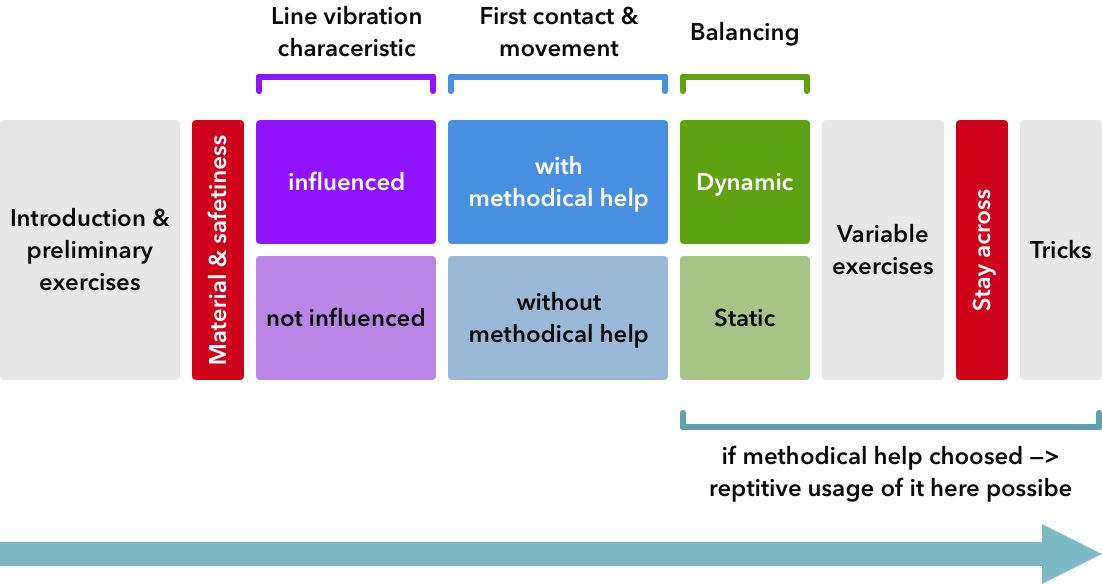
\includegraphics[width=0.91\linewidth]{Pictures/3_3_1_methodicalRoutine3}
		\caption{Methodical routine, adapted from Thomann~\cite{Thomann2013-aa}}
		\label{fig:3_3_1_methodicalRoutine}
	\end{minipage}
\end{figure}

\subsubsection{Differential method}
The differential or dynamic method follows another approach. It is in coherence with an open learning situation~\cite{Thomann2013-aa}. This means it depends on several factors, which in slacklining would be line type and length, tension, environment, etc. Considering the interplay of these factors each trainee can construct her own training set.
%Considering the interplay of these factors each trainee can reach the training goal by constructing her own training set.
A dynamic method is a practical usage for this~\cite{Beck2008-dl, Schoellhorn1999-ip}. This inherits the model of stepping stones. In general it describes that many ways can lead to the same goal. Each potential way has therefore its own level of difficulty. This results in a more modular way to reach a specific goal. In comparison to the methodical routine it leads to bigger differences in stimulus and provides more variability in the movement execution, like compared in Figure~\ref{fig:3_3_1_comparisonMethods}. 

\begin{figure}[htb]
	\centering
	\begin{minipage}[t]{1\linewidth}
		\centering
		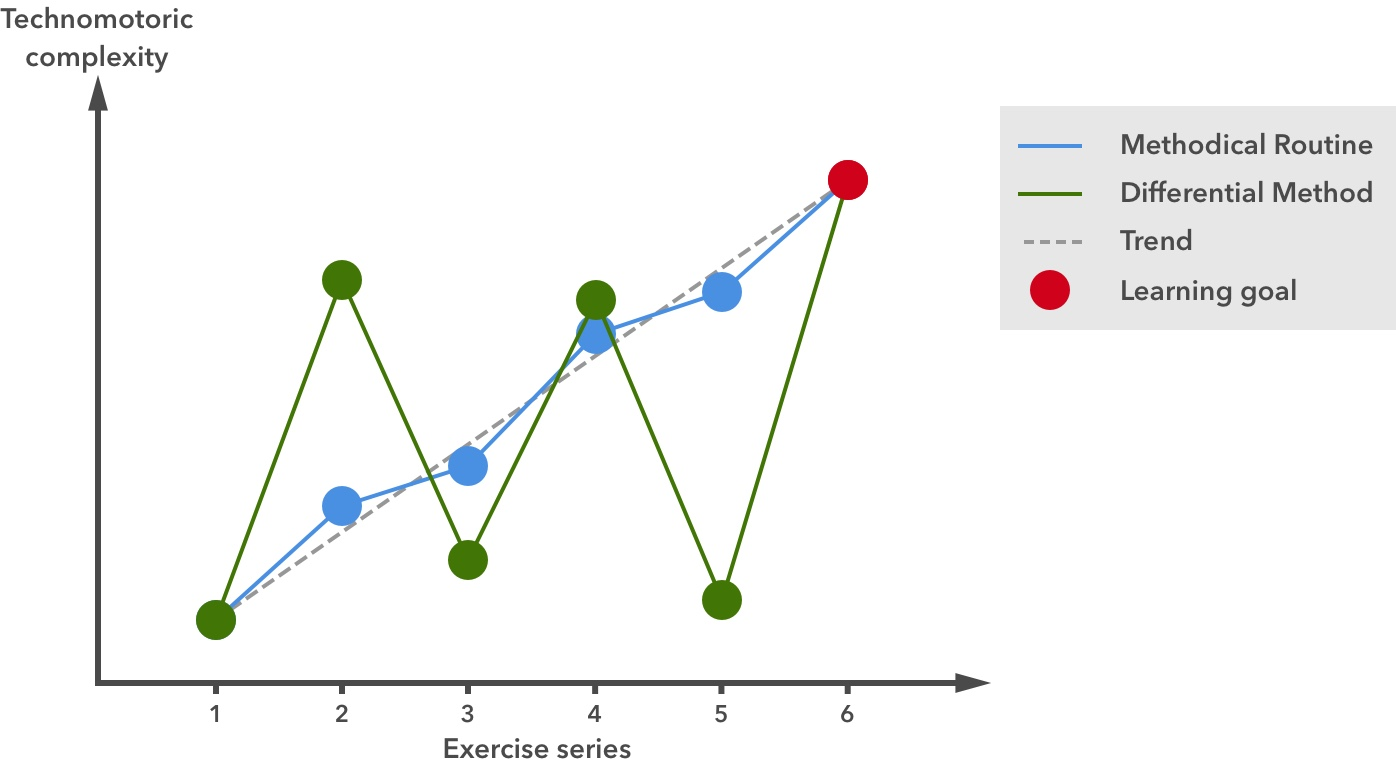
\includegraphics[width=1\linewidth]{Pictures/3_3_1_comparisonMethod2}
		\caption{Comparison methodical routine vs. differential method, adapted from Thomann~\cite{Thomann2013-aa}}
		\label{fig:3_3_1_comparisonMethods}
	\end{minipage}
\end{figure}
To make use of the differential learning method, the trainee can follow a methodical principle like seen in the methodical routine. If she reaches a certain skill level, more dynamic procedures can then be involved in the actual learning process. %Therefore the principle of differential learning can be used, which results in big stimulus differences and provide more variability in the movement execution.

The usage in slacklining can be integrated like described and visualized by Thomann~\cite{Thomann2013-aa} (Figure \ref{fig:3_3_1_dynamicMethod}). He divided exercises regarding to five learning stages and their coordinative demands and complexity. The main goal is to master controlled and complex movements on the line. The trainee has to choose an amount of various exercise of all stages. More complex exercises can either be supported by methodical help or the trainee can return to the lower stage to learn the movement for the specific exercise. Each trainee can therefore create her individual training path. Modification and integration of more useful exercises are allowed. Structured examples can be seen in Figure~\ref{fig:3_3_1_dynamicMethod}. The purple arrows visualize a way for more skilled people that are more coordinative, more venturesome, or have background knowledge. In contrast the green arrows visualize a path for more novice people that are less coordinate, less venturesome, or have no background knowledge in slacklining.
\begin{figure}[htb]
	\centering
	\begin{minipage}[t]{1\linewidth}
		\centering
		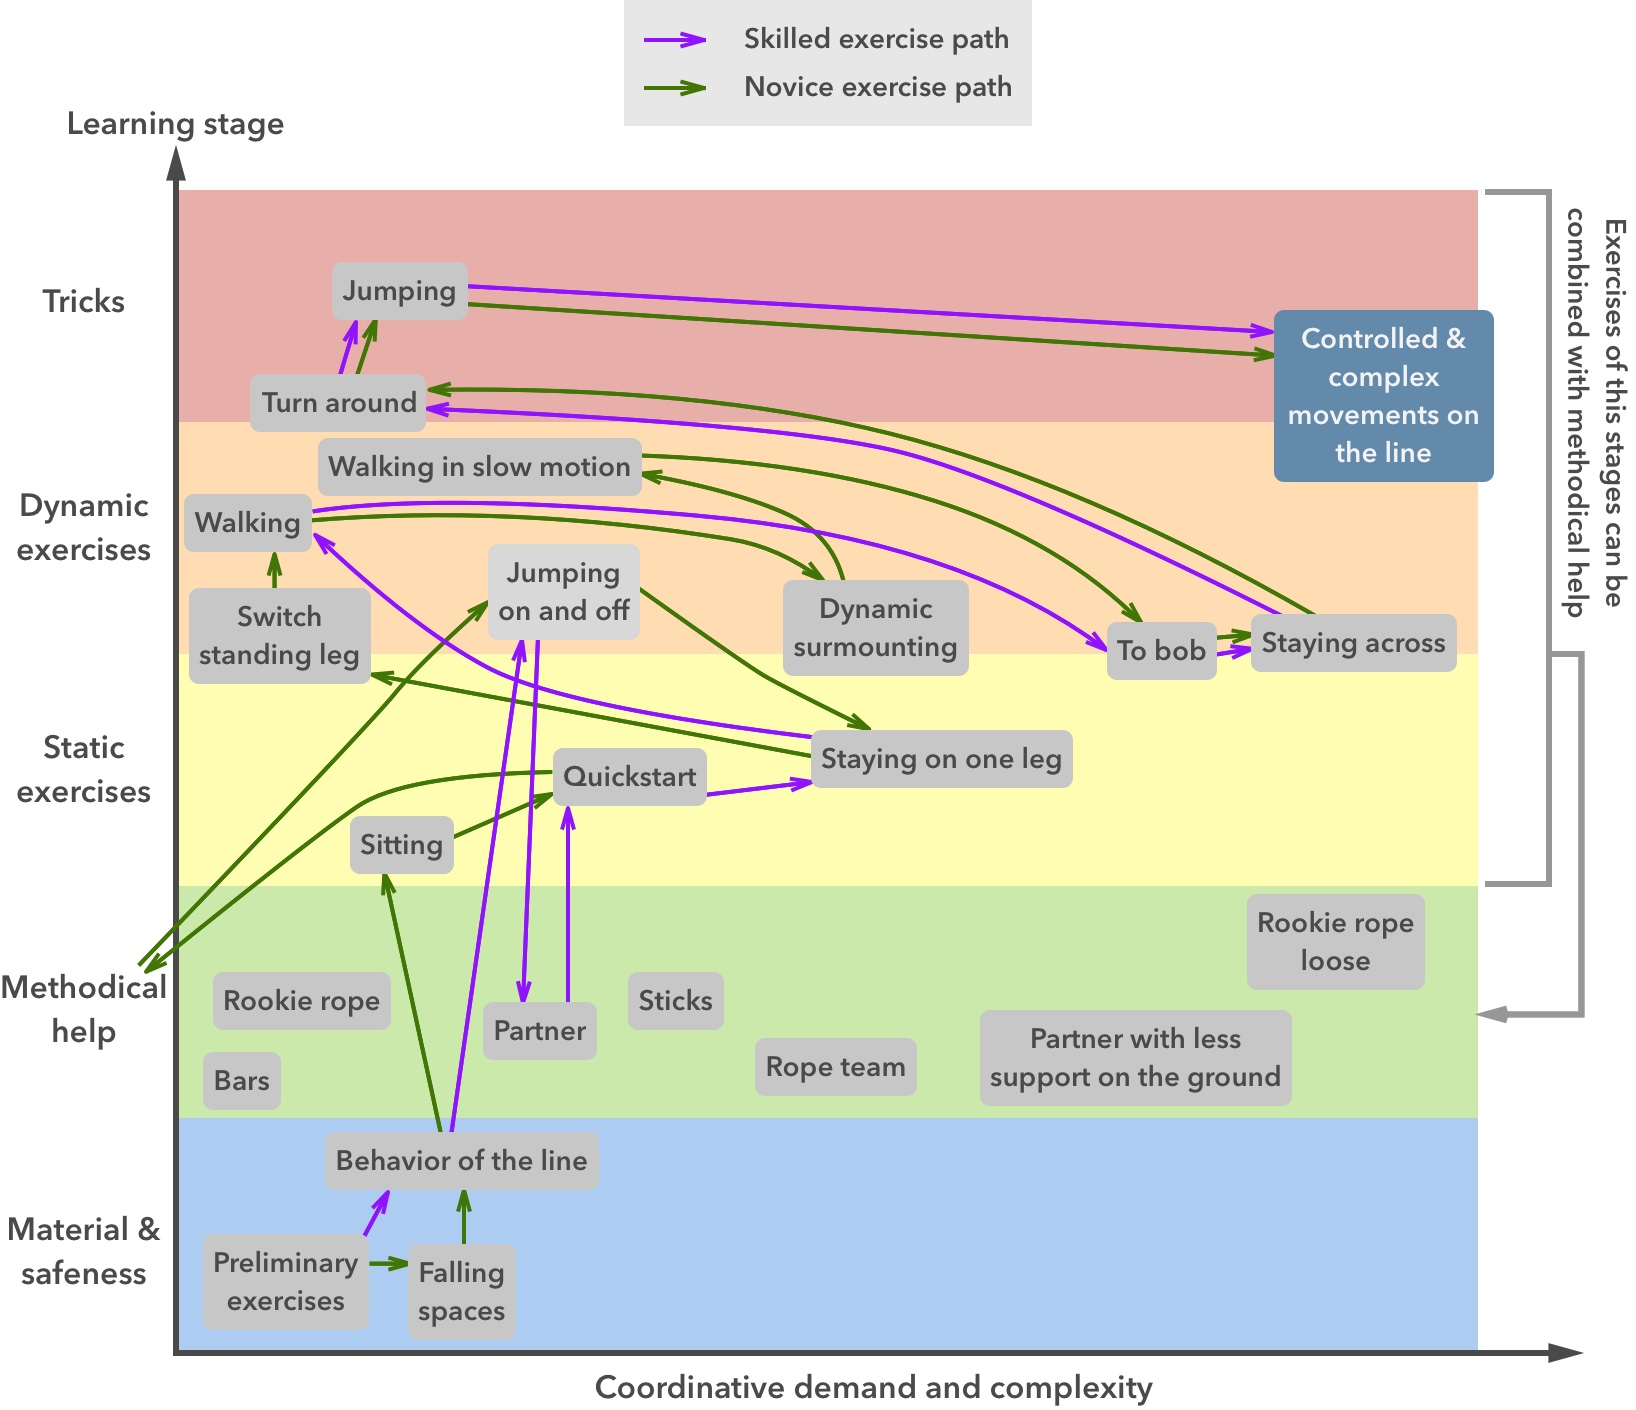
\includegraphics[width=1\linewidth]{Pictures/3_3_1_dynamicMethodBoth2}
		\caption{Dynamic methodic in slacklining, adapted from Thomann~\cite{Thomann2013-aa}}
		\label{fig:3_3_1_dynamicMethod}
	\end{minipage}
\end{figure}

For proper training with the system the trainee should follow a clear workflow. Therefore the methodical routine is the better choice as a learning concept in this interactive learning system. She learns right from the beginning essential aspects of slacklining that are relevant and build up on each other. Because it follows a strict linear sequence, stages and exercises can be designed as levels and the implementation is more simple as a first approach of such a learning system. 
%The trainee can unlock further levels by successfully executing the prior exercise. 
The next subsection \textit{\nameref{3_3_2_StagesExercises}} will cover a clear workflow integration of exercises for this learning system.

\subsection{Levels and Exercises of Learning Slacklining}\label{3_3_2_StagesExercises}
% Drei verschiedene Grundfertigkeiten: zunächst muss man auf einem Bein stehen können, dazu kommt die schmale Unterstützungsfläche, auf der man balancieren soll. Nicht zuletzt befindet man sich in einer gewissen Höhe und nicht mehr auf sicherem Boden.
%Now that an overview about slacklining and its learning techniques are given several practical exercises have to be considered. 
Repetitive trials are one approach of learning to walk on the line. However, this could result in dangerous situations and frustration for the slacker because of her missing skills. Therefore, a set of slacklining exercise can teach and guide the trainee appropriately. It pursues the goal to balance in a controlled manner on the line, stand on it for a few seconds, and be able to walk a few steps. 

In general, three core skills have to be acquired to achieve this goal~\cite{Kroiss2007-ab}. At first, the slacker should be able to stay on one foot. This is essential because most of the time one foot serves as standing foot on the line and the other one as balance element. Second, balancing on a narrow surface is important since the slackline exists of a limited width. Lastly, she should manage the height due to the fact that a slackline is tensioned around the height of the knee and above.

Kroiß~\cite{Kroiss2007-ab} defined a useful execise set for slackline skill acquisition, which will be used as groundwork within the SLS. He elicited learning exercises for beginners on a slackline within a school class, which gives a structured basis on the exercise integration. Further, several other works~\cite{Balcom2005-wl, Donath2013-kk, Donath2016-gm, Granacher2010-ow, Keller2012-xh, Kleindl2011-bl, Pfusterschmied2013-yy, Thomann2013-aa} integrated similar exercises for their slackline training approach. The exercises implemented in this thesis have been categorized into four levels, which represent the fundamental basis of the exercise routines. In the following, each level is introduced, its goal clarified, and the learning aspects described:

\subsubsection{Level for Slacklining Skill Acquisition}
The first level serves as a preparation for the subsequent levels.
Preliminary exercises will be executed on the ground and thus no slackline is needed.
With this, the overall physical balance of the user will be strengthened.
The trainee learns how to use her arms as a balance function, set a focus point to calm the visual sense, and to execute exercises slowly and controlled to prevent and handle unpredictable body behaviour.
%In almost all exercises of this tier, the arms have to be stretched to the side, over the shoulder, and bent in about 135 degrees.
%This is the most important balance function because the slacker has freedom in all directions and can shift her body's center of gravity with this.
%Keeping the head up and setting a focus point can help to calm the visual sense of balance.
%Further all exercises should be executed slowly and controlled to be able to handle the unpredictable behaviour of the body.
%In general it is recommended to train barefoot or with socks to get a better feeling in the foots. The knees should be bent to have a better initial position for movement compensation.

Mastering the preliminary exercises leads the slacker to her first experience with the slackline.
The goal is to get a feeling for the slackline, to be able to get up on the line, as well as to hold herself for a short amount of time on the line.
This can be achieved by becoming familiar with the line, feeling the imbalance and how her body behaves, and getting a better feeling for counterbalancing unpredictable movements.
%She learns how to use the sweet spot of the line for a more comfortable vibration characteristic, aligning the foot always with the slackline, and having a relaxed but straight upper body to have a better initial positioning.
%Therefore starting at the sweet spot can help, which It is in about 1/3 of the line and an area with a comfortable vibration characteristic.
%The foot should also be always in alignment with the slackline to have the biggest amount of the sole covered with the line.
%This results in more contact area of the foot. %A relaxed but straight upper body can further help to hold the right position.

After finishing the second level the slacker is familiar with the line and able to get up the line.
The goal of the third level is to make her more confident with standing and prepare her for walking on the line.
All prior learned techniques prepared the trainee to this goal and have to be directly applied.
Hereby she has to make more usage of the balancing leg, which servers as an additional balancing parameter beside the arms.
%balancing leg comes now more into action. It serves as an additional balancing parameter to support the arms. 
%If the slacker has problems with going up on the line, she can keep the balancing leg vertically in line with the standing leg while going up and then move it to the side. The pressure is mostly around the ball of the foot.

More dynamical exercises are part of the last level.
The slacker should now be able to stand confidently on the line with one foot as well as with both feet.
Its goal is to teach how to make first steps as a result for walking on the line.
In general several static exercises, like getting up, balancing with one foot, and standing with both feet on the line have to be applied together.
%While staying on the line and when the slacker wants to make a step she can guide her balancing foot to the side of the line and shift it then forwards. Letting the knees together when making a step forward helps because the legs can support each other. Making small steps won't shift the body's center of gravity that much forward, which results in more control.
